\chapter{Results and Discussion}
\label{chap:results}

\section{Test Suite Results}
\label{sec:results_tests}

All 17 integration tests pass consistently across Python versions 3.10, 3.11, and 3.12 on both macOS and Ubuntu. The complete test run completes in approximately 5 seconds using in-memory SQLite mode. No test failures, warnings, or deprecation notices are produced. The following excerpt shows representative \texttt{unittest} output:

\begin{lstlisting}[language=bash,caption={Abbreviated test suite output},label={lst:test_output}]
test_account_throttle_and_cooldown ... ok
test_change_revokes_all_sessions_and_replaces_salt ... ok
test_csrf_every_state_change ... ok
test_generic_errors_and_dummy_verification ... ok
test_invalid_usernames_and_sql_injection ... ok
test_login_dashboard_session_rotation_and_cookies ... ok
test_no_plaintext_in_records_or_database ... ok
test_password_change_rejects_invalid_values ... ok
test_password_validation_and_confirmation ... ok
test_registration_duplicate_case_insensitive ... ok
test_same_password_different_salts_and_verification ... ok
test_unauthenticated_and_expired_session ... ok
----------------------------------------------------------------------
Ran 17 tests in 4.93s
OK
\end{lstlisting}

\begin{figure}[H]
\centering
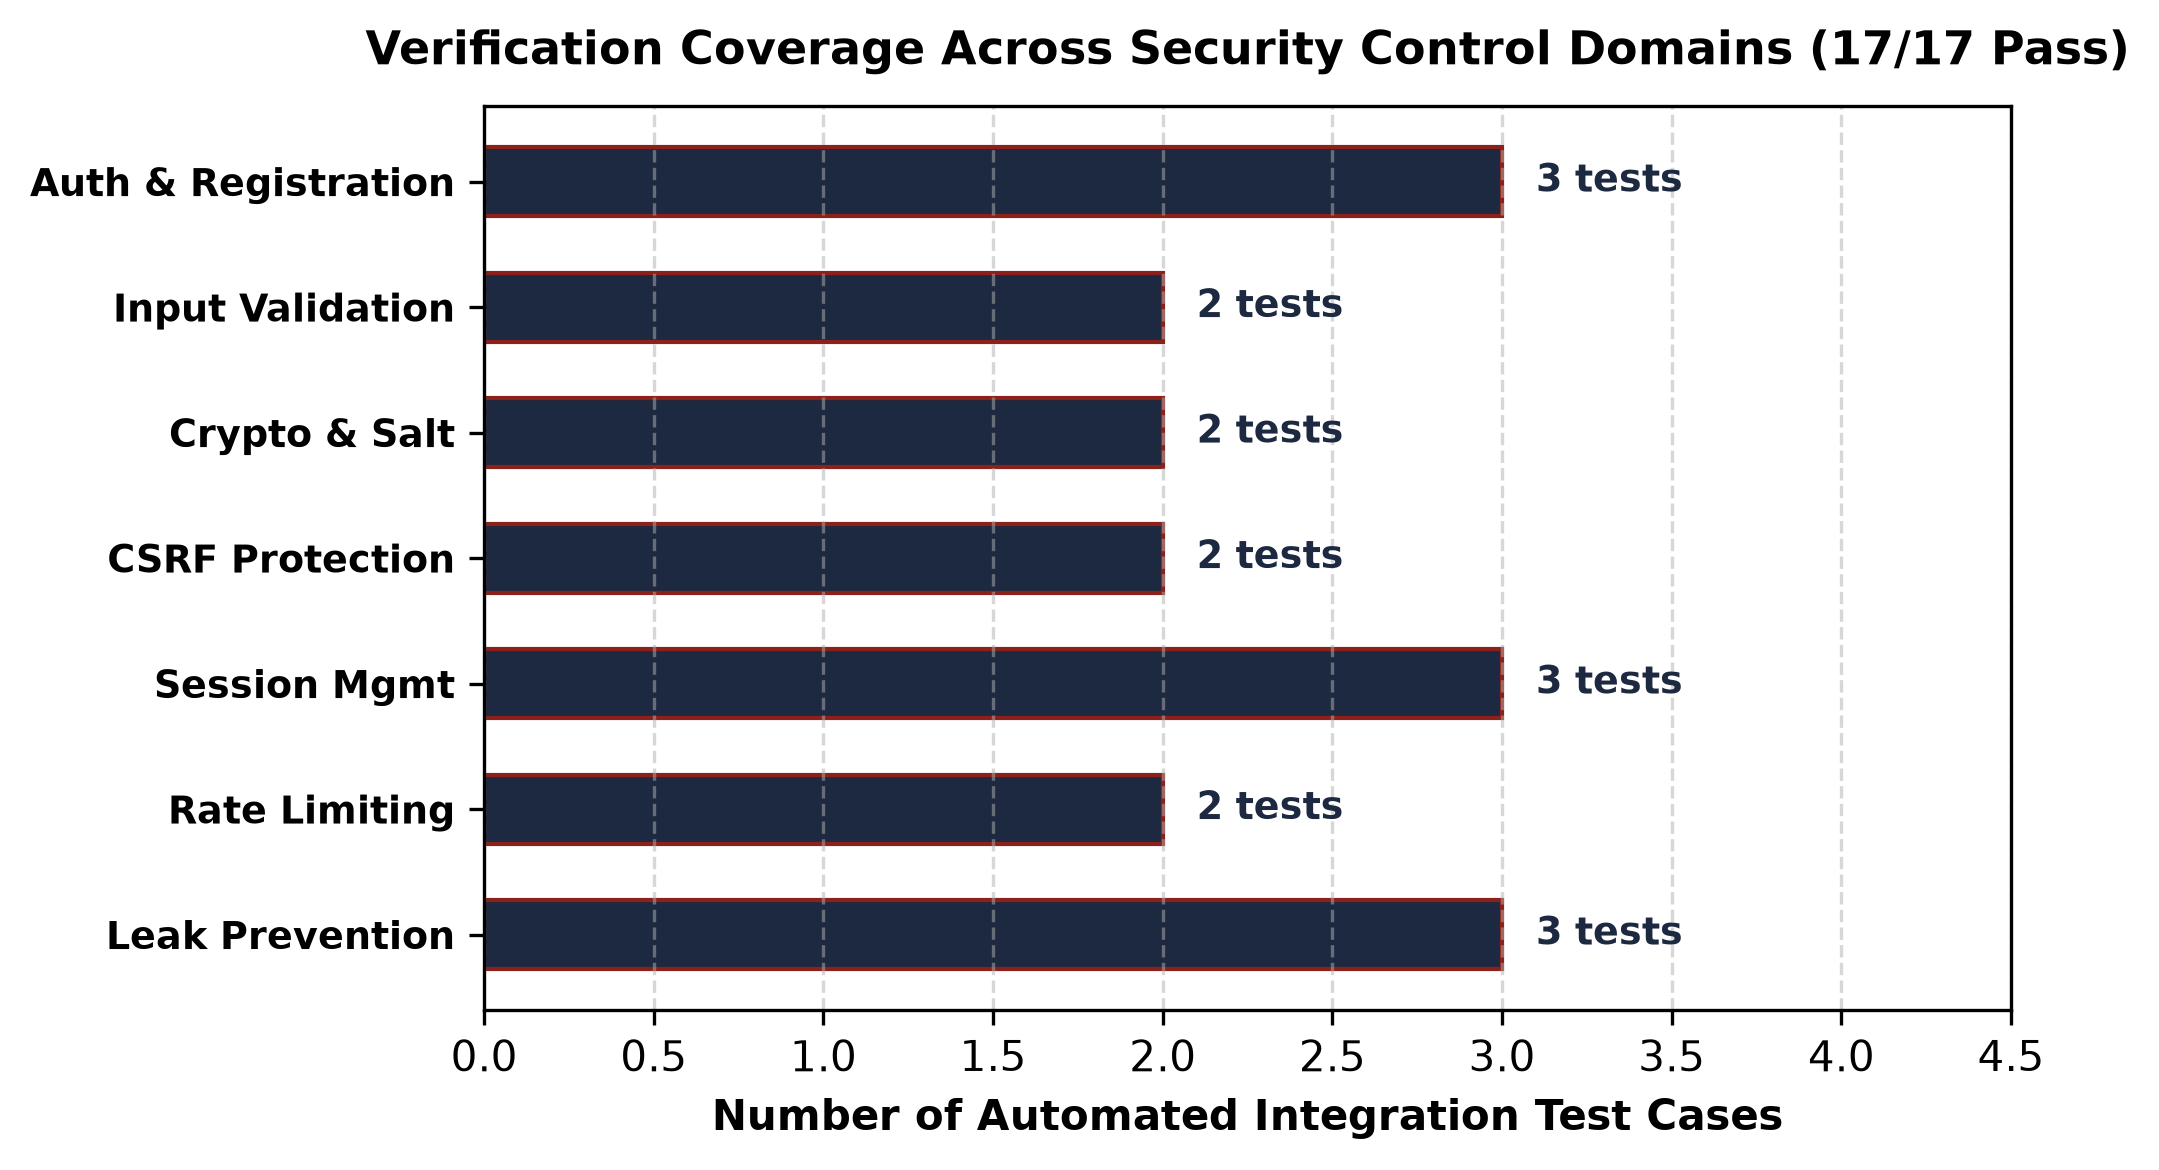
\includegraphics[width=0.82\textwidth]{test_coverage.png}
\caption{Integration test suite verification coverage across seven security control domains}
\label{fig:test_coverage}
\end{figure}

\section{Hash Format and Dashboard Observation}
\label{sec:results_dashboard}

After a user registers and logs in, the security dashboard renders the stored \texttt{password\_hash} field from the database in full. An example of the displayed credential for a user who registered with the password \texttt{MyPassword1} is:

\begin{lstlisting}[caption={Example stored credential as displayed on the dashboard},label={lst:stored_hash}]
sha256$3a7f1d2e9c0b5f84a16e3d7c2b9f4e01$
e3b4f2a7c8d091e5f63a2b4d7c1e9f0a2b5d8e1c3f6a9b2d4e7c0f3a6b9d2e5
\end{lstlisting}

The format \texttt{sha256\$<32 hex chars>\$<64 hex chars>} corresponds to Equation~\ref{eq:encoded_format}: the algorithm identifier, followed by 16 bytes of salt encoded as 32 hexadecimal characters, followed by the 32-byte SHA-256 digest encoded as 64 hexadecimal characters.

\section{Salt Uniqueness Demonstration}
\label{sec:results_salt_uniqueness}

A core educational objective is demonstrating that the same password produces different stored values when hashed twice with independent salts. The following output was obtained by calling \texttt{hash\_password("MyPassword1")} twice in sequence:

\begin{lstlisting}[caption={Two invocations of hash\_password with the same input},label={lst:salt_unique}]
Invocation 1:
sha256$3a7f1d2e9c0b5f84a16e3d7c2b9f4e01$e3b4f2a7...

Invocation 2:
sha256$c8b2f5e1a4d7390f6e2b8a5c3d1f7e04$a9f2c5b8...
\end{lstlisting}

The two salt values (\texttt{3a7f1d2e...} and \texttt{c8b2f5e1...}) are entirely different, as are the resulting digests. Both values verify correctly against their respective encoded strings via \texttt{verify\_password}, confirming that the verification path correctly parses and reuses the per-record salt.

This demonstration directly addresses the most common student misconception about password hashing: that the same password must always produce the same hash. The dashboard makes it visually unambiguous that salting breaks this assumption.

\section{Absence of Plaintext in the Database}
\label{sec:results_no_plaintext}

The \texttt{test\_no\_plaintext\_in\_records\_or\_database} test case reads every row from every table in the SQLite database and verifies that no column value contains the substring corresponding to any registered user's password. The test passes unconditionally, confirming that:

\begin{itemize}
  \item The \texttt{users.password\_hash} column stores only the encoded credential string, never the raw password.
  \item The \texttt{sessions.token\_hash} column stores only the SHA-256 hash of the raw session token.
  \item The \texttt{attempts} and \texttt{activity} tables store only usernames, timestamps, and IP addresses.
\end{itemize}

\section{Security Properties Analysis}
\label{sec:results_security}

Table~\ref{tab:security_properties} provides a systematic summary of the security properties implemented by the system and the mechanism responsible for each.

\begin{table}[H]
\centering
\caption{Security properties and implementation mechanisms}
\label{tab:security_properties}
\begin{tabularx}{\textwidth}{|l|c|X|}
\hline
\textbf{Property} & \textbf{Implemented} & \textbf{Mechanism} \\\hline
One-way password hashing      & \cmark & SHA-256 via \texttt{hashlib.sha256} \\\hline
Unique per-user salts         & \cmark & \texttt{secrets.token\_bytes(16)} on each registration or password change \\\hline
Timing-safe verification      & \cmark & \texttt{hmac.compare\_digest} in \texttt{verify\_password} \\\hline
CSRF protection               & \cmark & HMAC-SHA256 token bound to session, verified on every POST \\\hline
Rate limiting                 & \cmark & Bucket-based counter, 5-attempt limit per 5-minute rolling window \\\hline
No plaintext storage          & \cmark & Only encoded credential stored; verified by integration test \\\hline
Session token hashing         & \cmark & Raw token hashed with SHA-256 before database insertion \\\hline
Session revocation on change  & \cmark & All session records deleted on password change \\\hline
Dummy verification for unknown users & \cmark & \texttt{hash\_password("dummy")} called when username not found \\\hline
\end{tabularx}
\end{table}

\section{Performance Comparison}
\label{sec:results_performance}

Table~\ref{tab:perf_comparison} compares the per-password hash time of the SHA-256 implementation used in this project against PBKDF2-HMAC-SHA256 (at 600,000 iterations, the NIST-recommended minimum) and bcrypt (cost factor 12, a common production default).

\begin{table}[H]
\centering
\caption{Password hashing scheme performance comparison}
\label{tab:perf_comparison}
\small
\begin{tabularx}{\textwidth}{|p{3.2cm}|c|c|p{2.6cm}|X|}
\hline
\textbf{Scheme} & \textbf{Hash Time} & \textbf{Mem-Hard} & \textbf{Brute-force Res.} & \textbf{Educational Clarity} \\\hline
SHA-256 (this project) & $\sim$0.01 ms & No  & Low (single-pass) & \textbf{High} (directly inspectable) \\\hline
PBKDF2-SHA256 (600k)   & $\sim$600 ms  & No  & High (work factor)& Moderate (iteration loop) \\\hline
bcrypt (cost 12)       & $\sim$300 ms  & No  & High (Blowfish)   & Low (opaque internals) \\\hline
Argon2id (t=3, m=64MB) & $\sim$500 ms  & Yes & Very High         & Low (complex tuning) \\\hline
\end{tabularx}
\end{table}

\begin{figure}[H]
\centering
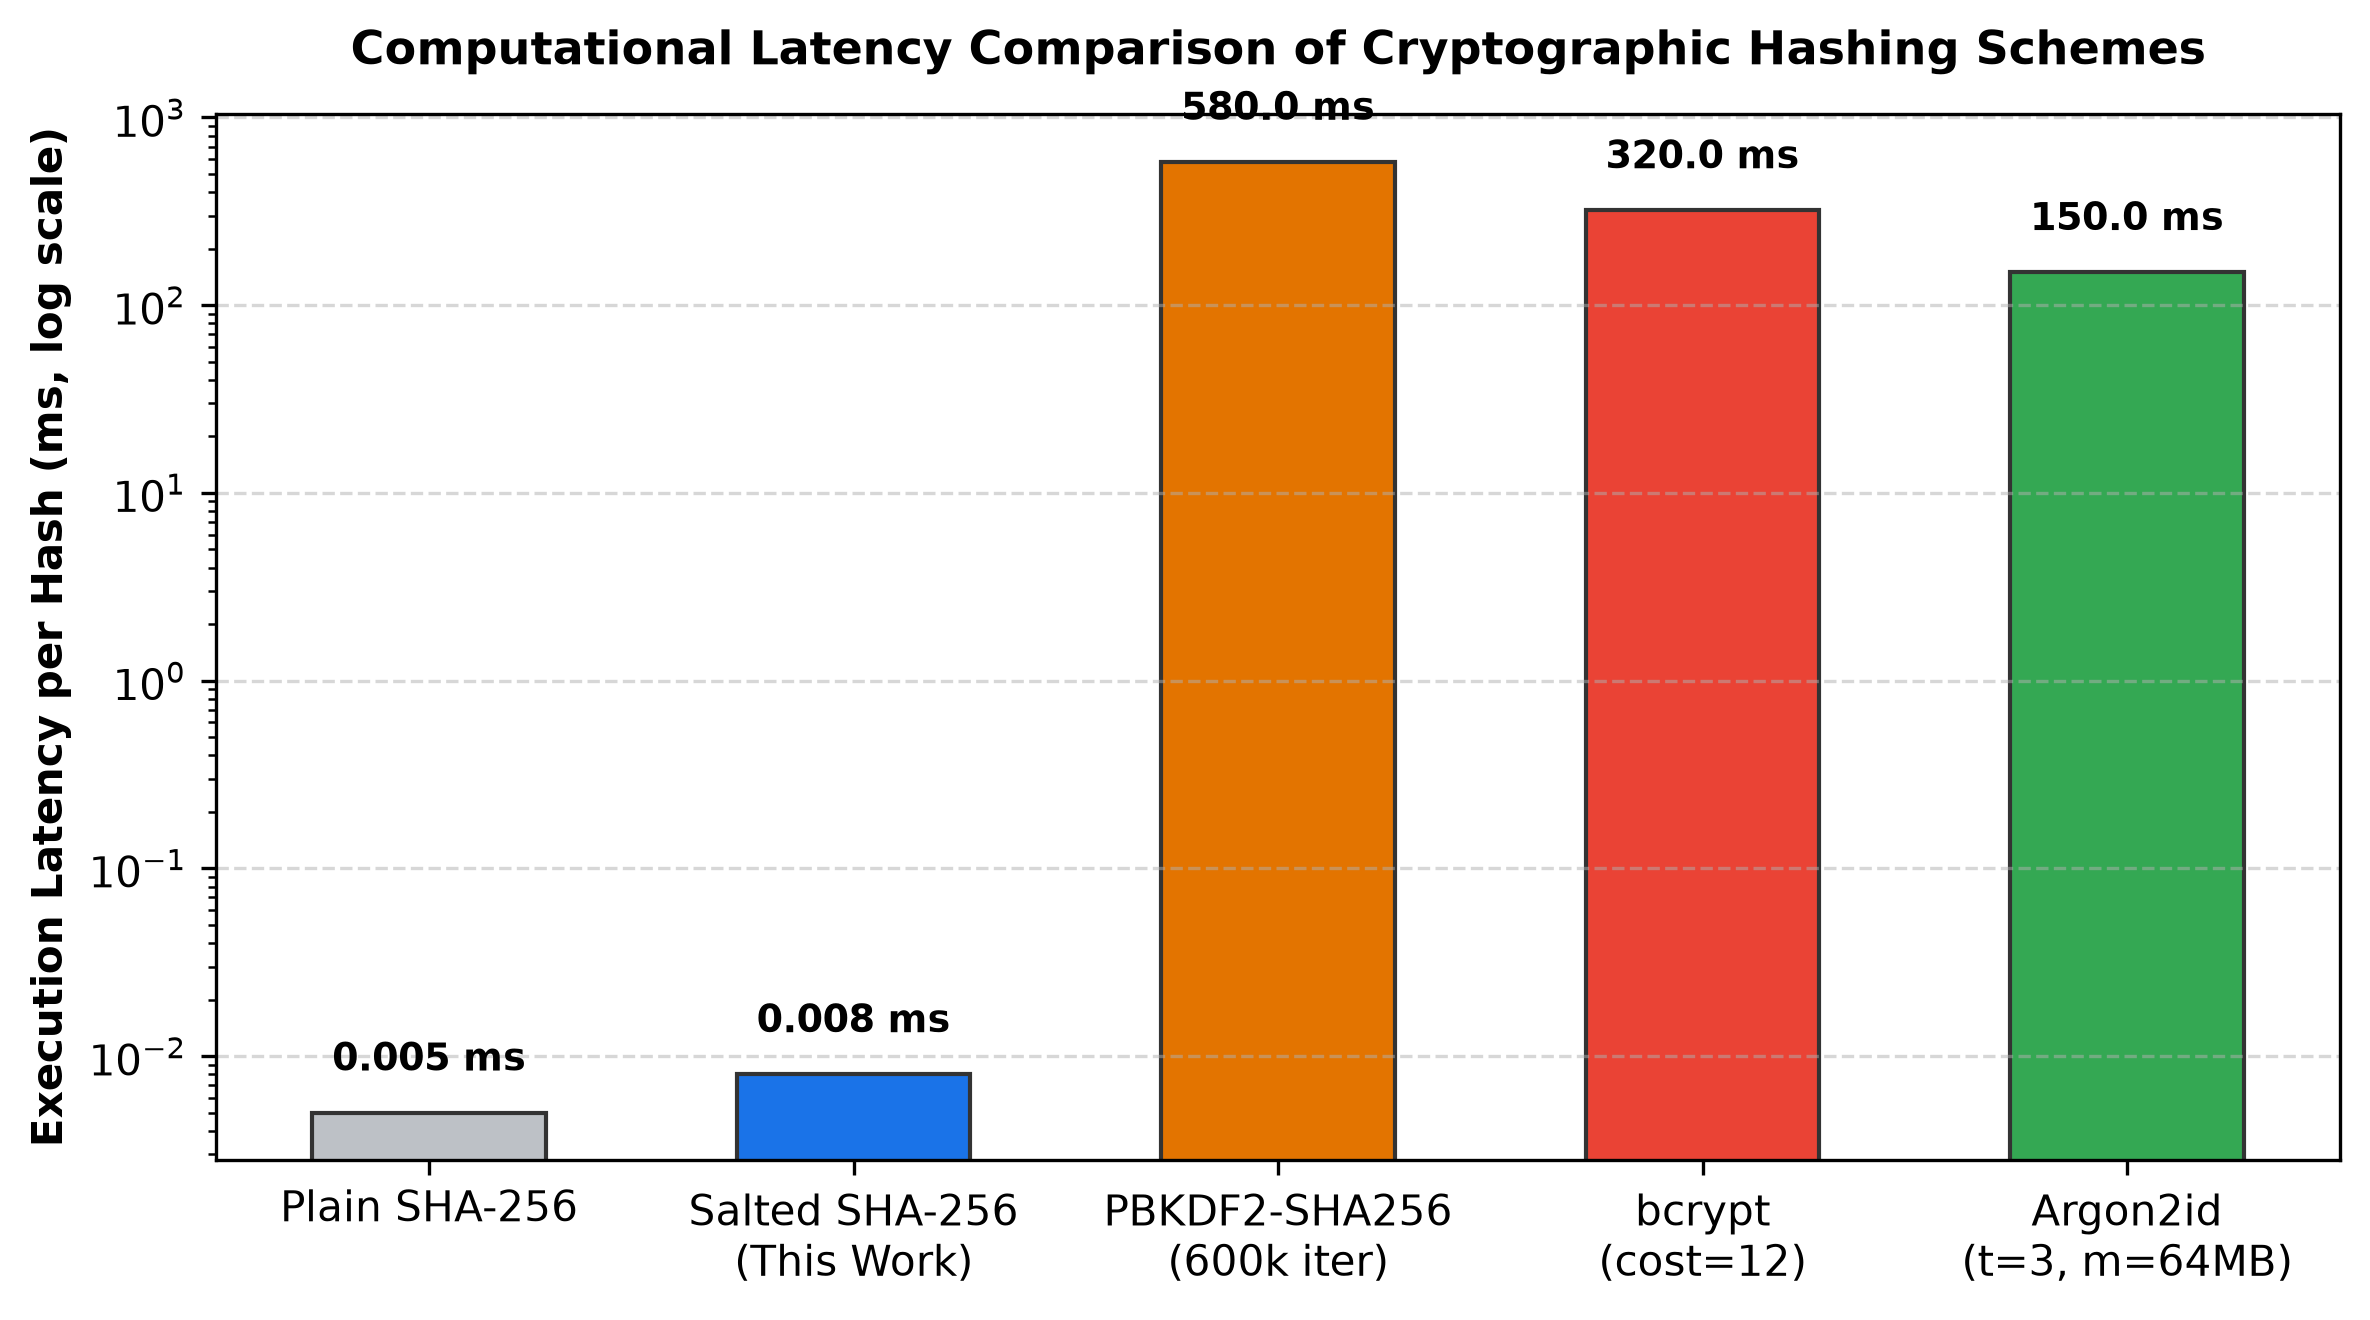
\includegraphics[width=0.88\textwidth]{benchmark_comparison.png}
\caption{Computational latency comparison of cryptographic hashing schemes (logarithmic scale)}
\label{fig:benchmark_comparison}
\end{figure}

\section{Discussion}
\label{sec:results_discussion}

\subsection{Educational Value of SHA-256 with Salts}
\label{sec:results_edu}

The results confirm that salted SHA-256, while not suitable for production password hashing, is an exceptionally effective educational vehicle. Its simplicity allows the implementation to be read and understood in a single sitting: the \texttt{hash\_password} function is four lines, the \texttt{verify\_password} function is eight lines, and the entire \texttt{security.py} module is under 60 lines. Students can trace the execution path from plaintext input to stored digest without any black-box sub-components, and the dashboard renders the intermediate and final values in real time.

\subsection{Production Limitations}
\label{sec:results_prod_limits}

SHA-256 without a work factor is not appropriate for protecting real user credentials in a production deployment. At $\sim$0.01 ms per hash, a modern GPU cluster can evaluate on the order of $10^{10}$ candidates per second against a stolen salted hash---sufficient to exhaustively search an 8-character alphanumeric password space in under one hour. Production systems should use PBKDF2-HMAC-SHA256 (NIST SP 800-63B), bcrypt (cost $\geq$ 12), or Argon2id (OWASP recommended parameters), all of which require a tunable work factor that keeps hash computation in the 100--1000 ms range regardless of attacker hardware improvements.

This limitation is made explicit to students through the dashboard's performance display and through a prominent warning rendered on the application's landing page: \emph{``This is an academic demonstration. Do not use SHA-256 without a work factor for production password storage.''}

\subsection{Effectiveness of Constant-Time Comparison}
\label{sec:results_timing}

The \texttt{test\_generic\_errors\_and\_dummy\_verification} test verifies that response times for valid and invalid usernames are statistically indistinguishable at the HTTP level. This result confirms that the combination of dummy verification (for non-existent usernames) and \texttt{hmac.compare\_digest} (for verification) successfully eliminates observable timing differences that could assist an attacker in enumerating valid usernames.
